\documentclass[11pt]{article}

\usepackage{amsmath}
\usepackage{amssymb}
\usepackage{array}
\usepackage{geometry}
\usepackage{enumitem}
\usepackage{float}
\usepackage{cancel}
\usepackage{graphicx}
\usepackage[labelformat=empty]{caption}
\usepackage{booktabs}

\geometry{
	a4paper,
 	left=20mm,
 	top=20mm,
 	bottom=20mm,
}

\setlength{\parindent}{0pt}

\begin{document}

\section{Wahrscheinlichkeiten}

\begin{description}[labelindent=16pt,style=multiline,leftmargin=9cm, noitemsep]
	\item[Ereignisraum $\Omega$:] Die Menge aller m{\"o}glichen Ergebnisse
	\item[Elementarereignis $\omega \in \Omega$:] Elemente vom Ereignisraum
	\item[Potenzmenge $\mathcal{P}(\Omega)$ oder $2^\Omega$:] Menge aller Teilmengen von $\Omega$
	\item[prinzipielles Ereigniss $A \subseteq \Omega$:] Kollektion von Elementarereignissen
	\item[Klasse der beobachtbaren Ereignisse $\mathcal{F}$:] Teilmenge der Potzenmenge $\mathcal{P}(\Omega)$ (alle m{\"o}glichen Ereignisse)
	\item[Wahrscheinlichkeitsmass $P: \mathcal{F} \mapsto \lbrack 0,1 \rbrack $:] Weist einem Ereignis eine Wahrscheinlichkeit zu
\end{description}

Es gelten:
\begin{equation*}
\begin{split}
	P[A \cup B] & = P[A] + P[B] - P[A \cap B] \quad\text{(Additionsregel)} \\
	P[A \cap B] & = P[B|A] \cdot P[A] \quad\text{(Multiplikationsregel)} \\
	P[A \backslash B] & = P[A] - P[A \cup B] \\
\end{split}
\end{equation*}

\subsection{Diskrete Wahrscheinlichkeitsr{\"a}ume}

Ist $\Omega = {\omega_1, \omega_2,...,\omega_N}$ endlich mit $|\Omega| = N$ und $\mathcal{F} = 2^\Omega$ und sind die Elementarereignisse alle gleich wahrscheinlich, so ist $\Omega$ ein \textbf{Laplace-Raum} und $P$ die \textbf{diskrete Gleichverteilung} auf $\Omega$.

\begin{equation*}
	P[A] = \frac{\text{Anzahl der Elementarereignisse in A}}{\text{Anzahl der Elementarereignisse in $\Omega$}} = \frac{|A|}{|\Omega|}
\end{equation*}

\subsection{Bedingte Wahrscheinlichkeiten}

Die bedingte Wahrscheinlichkeit von $B$ unter der Bedingung, dass $A$ eintritt ($A$ gegeben) ist definiert durch:
\begin{equation*}
	P[B|A] := \frac{P[B \cap A]}{P[A]}
\end{equation*}

\emph{Veranschaulichung:} $A$ ist eingetreten. Da $A$ und $B$ von einander abh{\"a}ngen, l{\"a}sst sich somit auch die Wahrscheinlichkeit berechnen, dass $B$ eingetreten ist.

\paragraph{Satz der totalen Wahrscheinlichkeit:} Sei $A_1,...,A_n$ eine Zerlegung von $\Omega$ in paarweise disjunkte Ereignisse, dann gilt f{\"u}r ein beliebiges Ereignis $B$:
\begin{equation*}
	P[B] = \sum_{i=1}^n P[B|A_i] P[A_i]
\end{equation*}
\begin{center}
	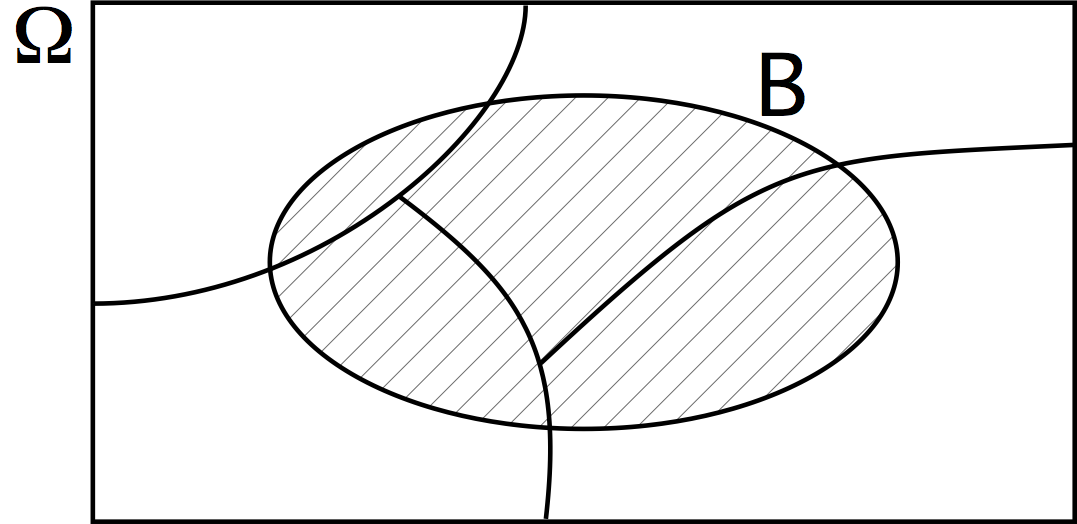
\includegraphics[width=200pt]{images/totale_wahrscheinlichkeit}
\end{center}

\paragraph{Formel von Bayes:} Ist $A_1,...,A_n$ eine Zerlegung von $\Omega$ mit $P[A_i] > 0$ und $B$ ein Ereignis mit $P[B] > 0$ so gilt f{\"u}r jedes $k$:
\begin{equation*}
	P[A_k|B] = \frac{P[B|A_k]P[A_k]}{\sum_{i=1}^n P[B|A_i]P[A_i]}
\end{equation*}

\subsection{Unabh{\"a}ngigkeit}

Zwei Ereignisse $A, B$ sind unabh{\"a}ngig (stochastisch), falls gilt:
\begin{equation*}
\begin{split}
	P[A \cap B] & = P[A]P[B] \quad\text{(Produktregel)}\\
	P[B|A] & = P[B] \\
	P[A|B] & = P[A] \\
\end{split}
\end{equation*}

\emph{Veranschaulichung:} Die Tatsache, dass eines der Ereignisse eingetreten ist, hat keinen Einfluss auf die Wahrscheinlichkeit des anderen.
	
\end{document}
